\chapter{Szabályozó modellezése}\label{chap:controller}

Az~\ref{chap:observer}.\ fejezetben levezetett állapotmegfigyelő és a szögelfordulás közvetlen mérése
együtt a rendszer teljes állapotvektorát elérhetővé teszi. Az impedancia modell által előírt dinamikai összefüggés
első lépésben teljes állapotvisszacsatolással biztosítható. A rendszer pólusai a~\ref{chap:controllability}.\ fejezetben
vizsgált irányíthatósági feltétel teljesülése miatt szabadon áthelyezhetők.

\section{Pozíció szabályozás}
Az előírt modell két független változót is tartalmaz, a pólusáthelyezés viszont egyetlen bemenetre 
alkalmazható. Jelen esetben a szögelfordulásra és a külső nyomatékra adott válasz csak az amplitúdóban
tér el. Ezt kihasználva először kizárólag a szögelfordulás referencia jelére előírt válasz alapján 
kerülnek áthelyezésre a pólusok. Teljes állapotvisszacsatolás esetén a motorra kapcsolt feszültség
\begin{align}\label{eq:position_control_voltage}
    V = \BF K \tilde{\BF x} + k_1 \theta_\RM r
\end{align}
összefüggéssel adható meg, 
ahol $\BF K$ az állapotvisszacsatolási mátrix, 
$k_1$ a az állapotvisszacsatolási mátrix első eleme és 
$\theta_\RM r$ az előírt szögelfordulás. Az~\eqref{eq:position_control_voltage} egyenletet felhasználásával
az~\eqref{eq:state_space_generic} állapottér modell belső állapotának dinamikája
\begin{align}\label{eq:position_control_law_state}
    \dot{\BF x} = \BF A \BF x + \BF B_\RM V\left[-\BF K \tilde{\BF x} + k_1 \theta_r\right] + \BF B_\RM \tau \tau_\RM e,
\end{align}
alakban írható át. A $\BF B$ mátrix oszlopai elkülönítve $\BF B_\RM V$ és $\BF B_\RM \tau$ paraméterekként jelennek meg.
Bevezetve a valós és becsült állapot közötti hibát, mint
\begin{align}
    \BF e = \BF x_\RM b - \tilde{\BF x}_\RM b,
\end{align}
az~\eqref{eq:position_control_law_state} egyenlet a becsült a állapotok vektorának kiküszöbölésével
\begin{align}
    \dot{\BF x} = \left(\BF A - \BF B_\RM V \BF K\right) \BF x + 
    \BF B_\RM V \BF K_\RM b \BF e + 
    \BF B_\RM \tau \tau + 
    \BF B_\RM V k_1 \theta_\RM r,
\end{align}
alakra hozható. A valós és becsült állapot közötti hiba dinamikája~\eqref{eq:observer_state} felhasználásával
\begin{equation}
    \begin{split}
    \dot{\BF x}_\RM b &= \BF A_\RM{ba} x_\RM a + \BF A_\RM{bb} \BF x_\RM b + 
    \BF B_\RM{Vb} V + \BF B_\RM{\tau b} \tau_\RM e\,,\\
    \dot{\tilde{\BF x}}_\RM b &= \left(\BF A_\RM{bb} - \BF K_\RM e \BF A_\RM{ab}\right) \tilde{\BF x}_\RM b +
    \BF A_\RM{ba} x_\RM a +
    \BF K_\RM e \BF A_\RM{ab} \BF x_\RM b +
    \BF B_\RM{Vb} V + \BF B_\RM{\tau b} \tau\,,
    \end{split}
\end{equation}
melyeket kivonva egymásból
\begin{align}
    \dot{\BF e} = \left(\BF A_\RM{bb} - \BF K_\RM e \BF A_\RM{ab}\right) \BF e\,.
\end{align}
A rendszer dinamikája blokk mátrix alakban
\begin{align}
    \begin{bmatrix}
        \dot{\BF x} \\
        \dot{\BF e}
    \end{bmatrix}
    =
    \begin{bmatrix}
        \BF A - \BF B_\RM V \BF K & \BF B_\RM V \BF K_\RM b \\
        \BF 0 & \BF A_\RM{bb} - \BF K_\RM e \BF A_\RM{ab}
    \end{bmatrix}
    \begin{bmatrix}
        \BF x \\
        \BF e
    \end{bmatrix}
    +
    \begin{bmatrix}
        \BF B_\RM \tau & \BF B_\RM V k_1\\
        \BF 0 & \BF 0
    \end{bmatrix}
    \begin{bmatrix}
        \tau \\
        \theta_\RM r
    \end{bmatrix}.
\end{align}

\begin{figure}[ht]
    \begin{center}
    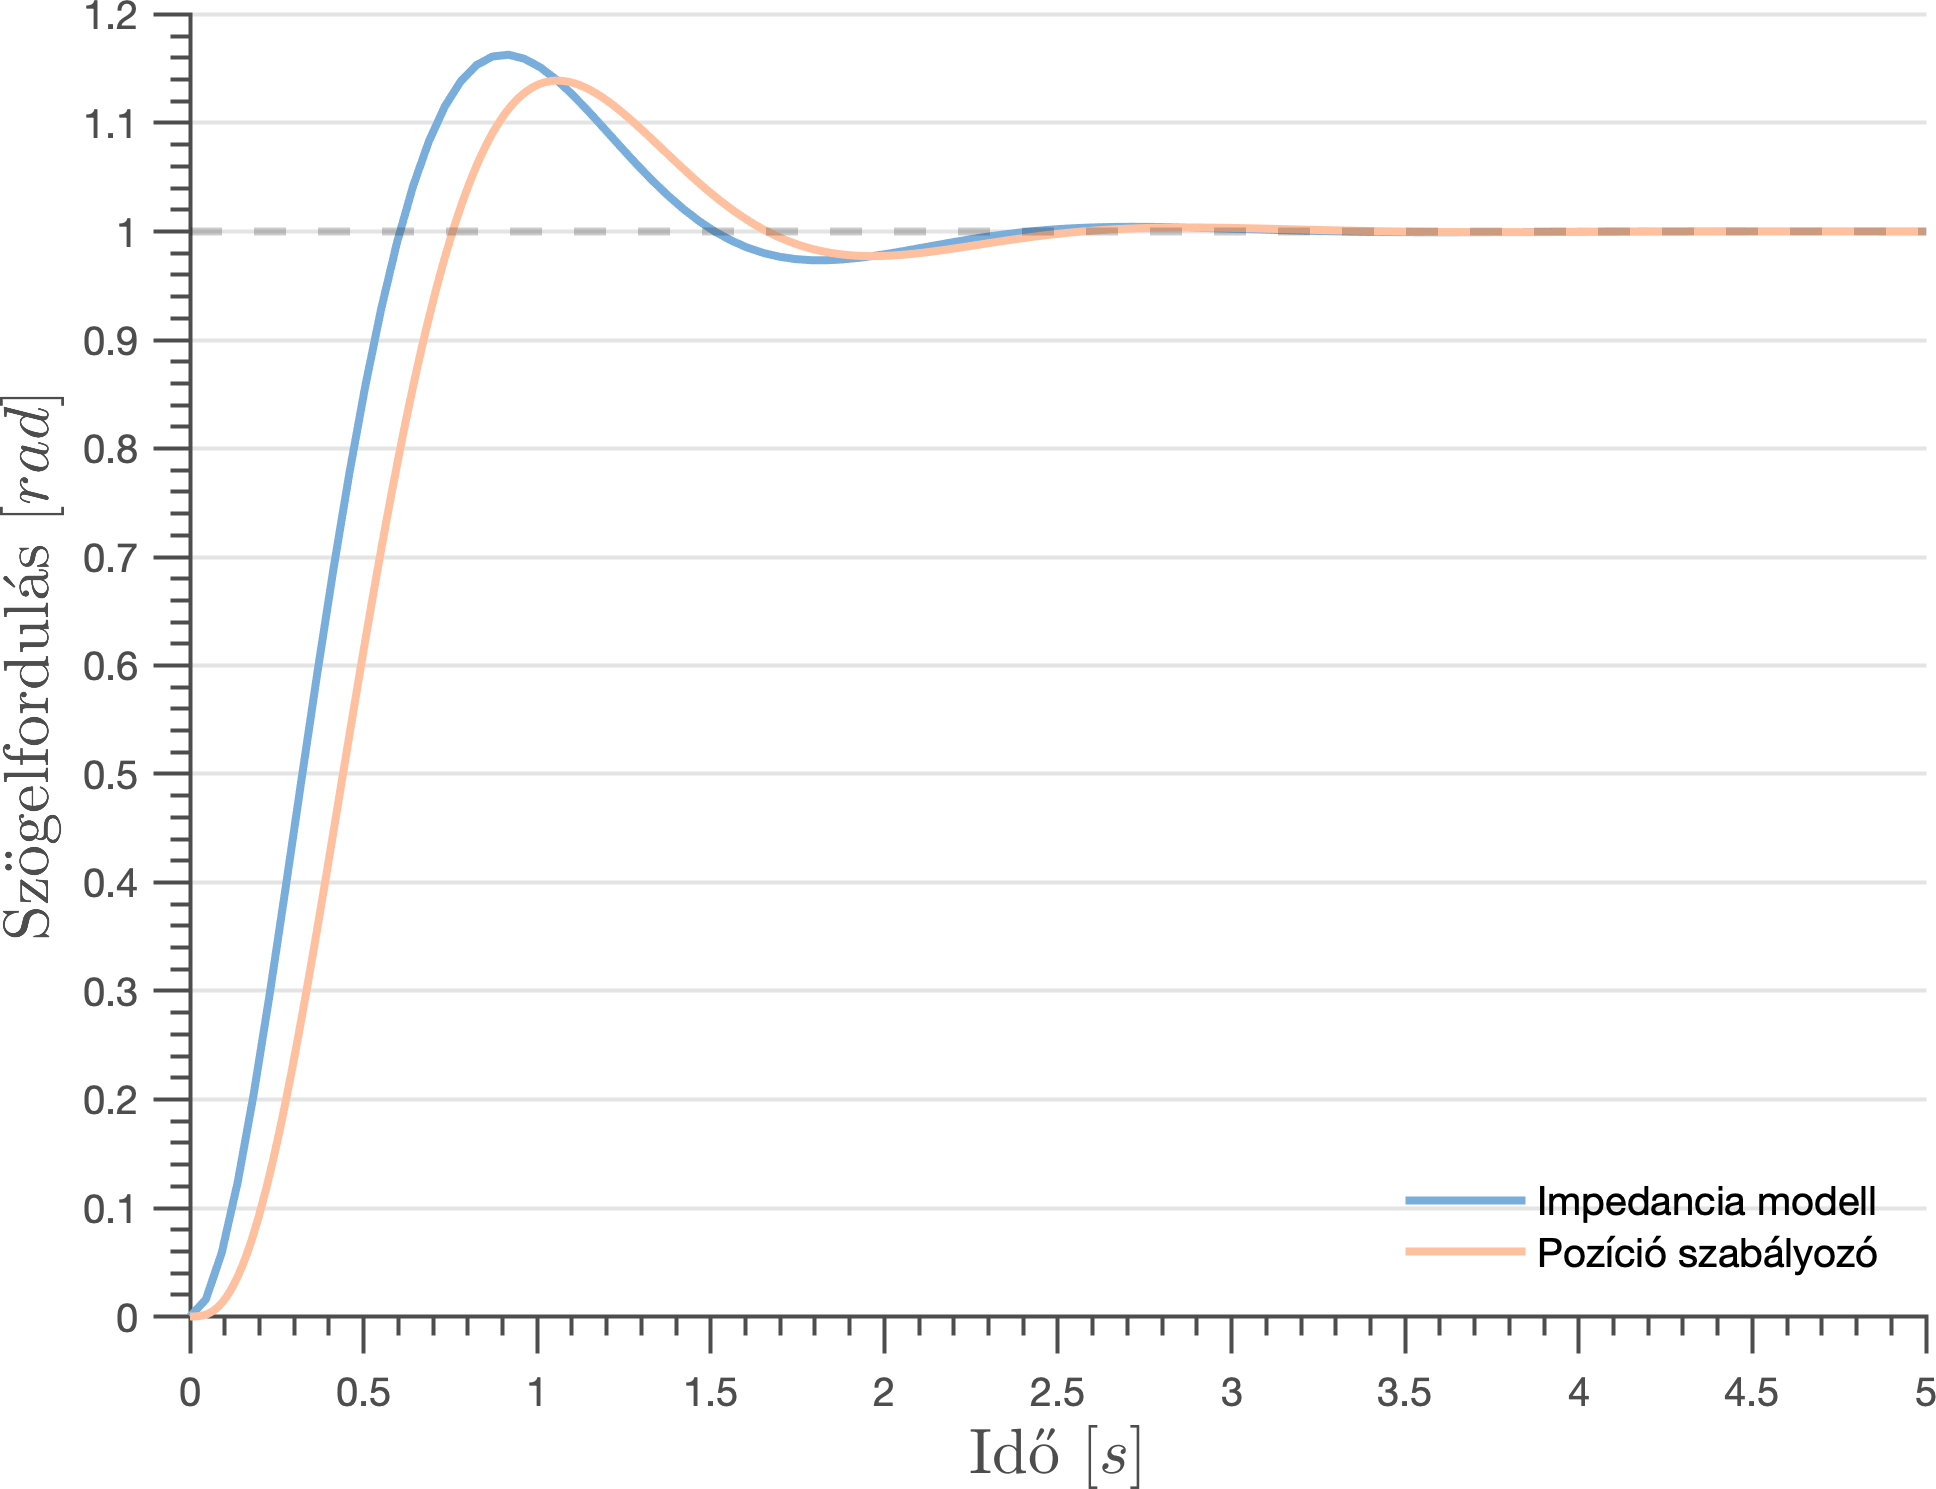
\includegraphics[width=\textwidth]{images/observer_controller_pos_resp.png}
    \caption{Az impedancia modell és a szabályozó összehasonlítása pozíció egységugrás bemenetre}\label{fig:observer_controller_pos_resp}
    \end{center}
\end{figure}

\begin{figure}[ht]
    \begin{center}
    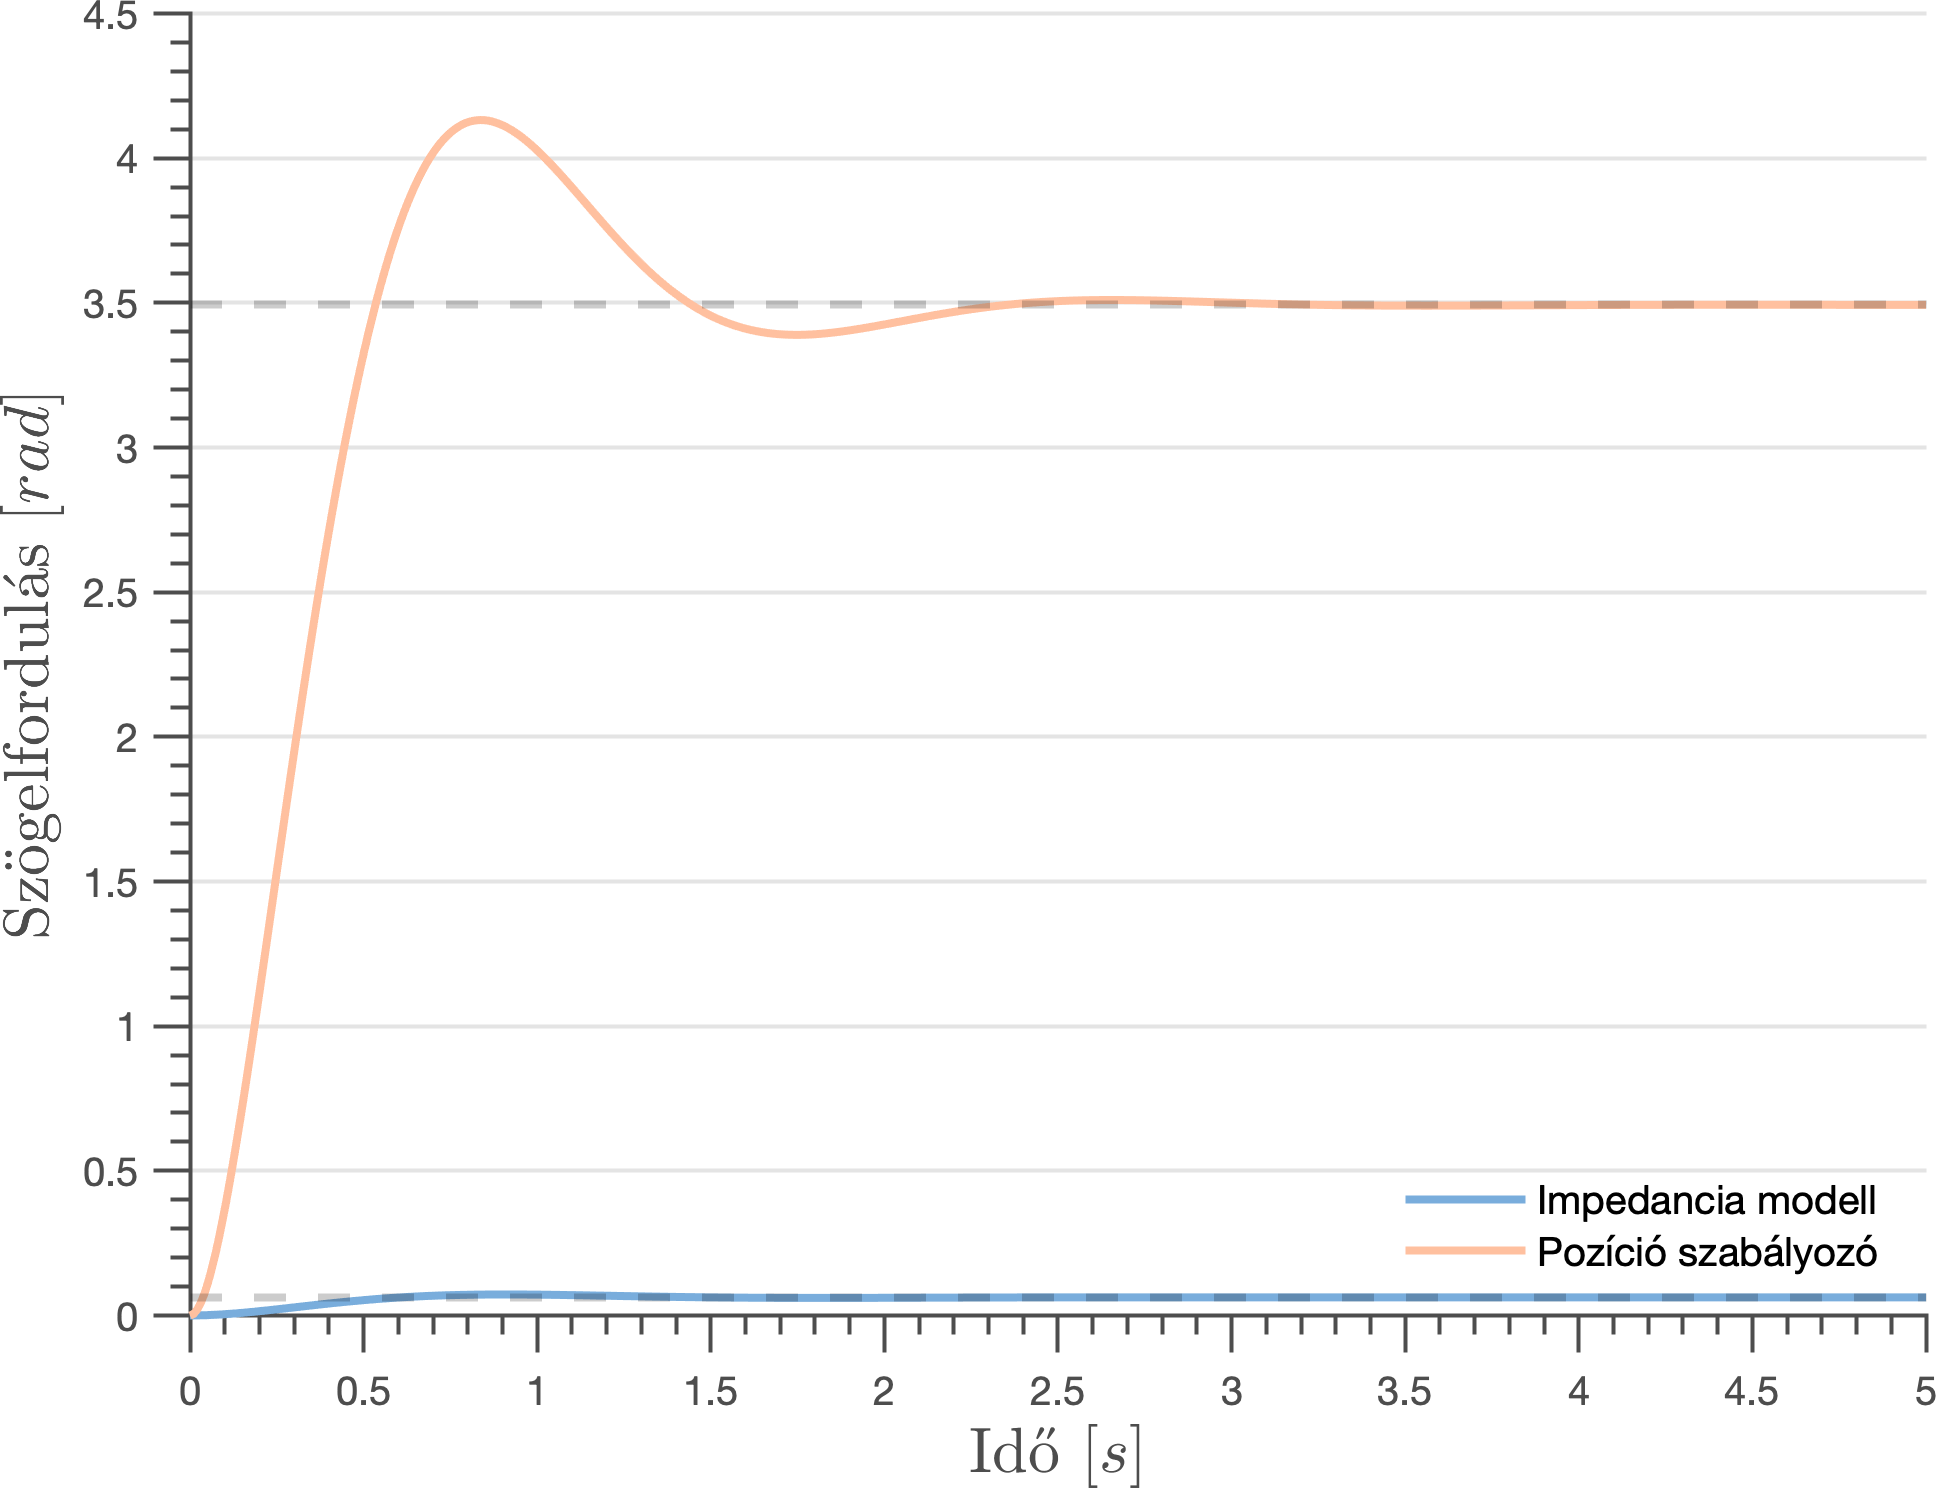
\includegraphics[width=\textwidth]{images/observer_controller_torque_resp.png}
    \caption{Az impedancia modell és a szabályozó összehasonlítása külső nyomaték egységugrás bemenetre}\label{fig:observer_controller_torque_resp}
    \end{center}
\end{figure}


\section{Nyomaték kompenzáció}
A modell két bemenete közül csak a feszültségre van hatással a 
szabályozó. A külső nyomaték környezeti hatásokból ered. Az impedancia 
modell mindkét bemenetre adott válasz alakját előírja, így a környezet 
hatását a feszültség megváltoztatásával kell kompenzálni. A kompenzáció
a külső nyomaték direkt vagy indirekt visszacsatolásával érhető el.
Direkt mérés esetén a külső nyomaték értékét egy szenzor adja meg, 
mely dinamikája jelen vizsgálat során elhanyagolható. Az
állapotmegfigyelővel és kompenzációval ellátott rendszer teljes 
blokkdiagramját az~\ref{fig:block_diagram_direct_compensation}-es ábra mutatja.
\begin{figure}[ht]
    \begin{center}
    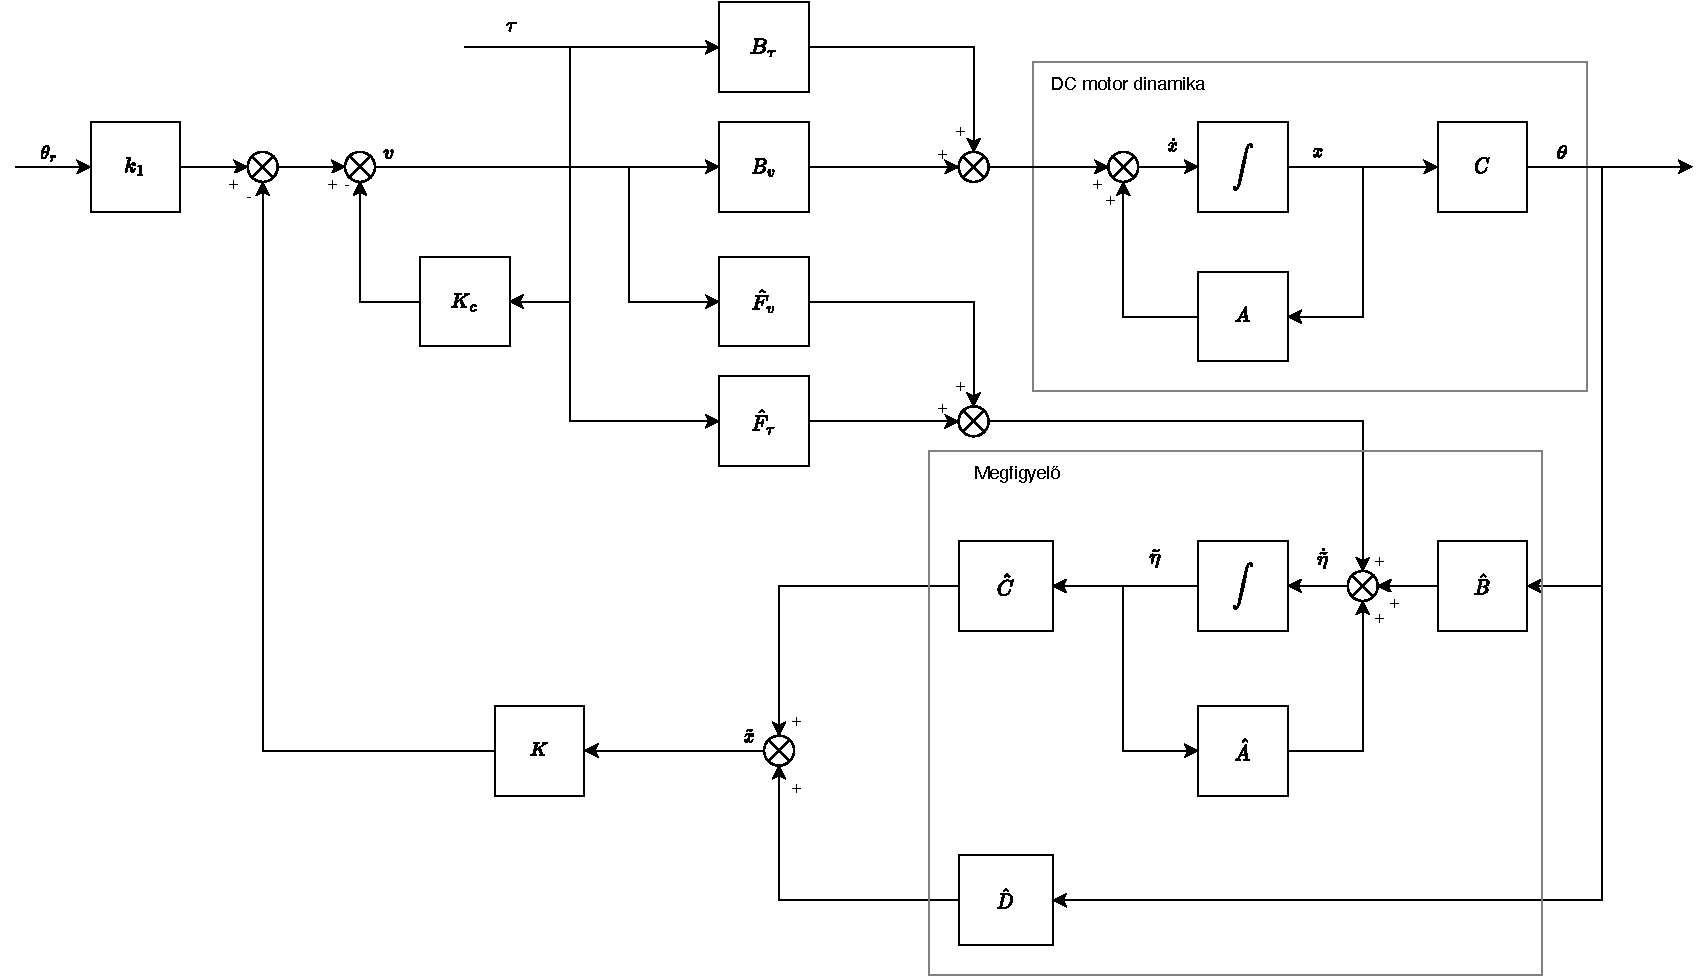
\includegraphics[width=\textwidth]{images/compensated_position_control_torque.drawio.pdf}
    \caption{Impedancia szabályozó közvetlen nyomaték méréssel}\label{fig:block_diagram_direct_compensation}
    \end{center}
\end{figure}
A teljes rendszer dinamikája az~\eqref{eq:state_space}-es állapottér modell és az ~\eqref{eq:observer}-es 
állapotmegfigyelő összekapcsolásával írható le, a következő visszacsatolási összefüggéssel
\begin{align}
    V = -\BF K \tilde{\BF x} -K_c \tau + k_1 \theta_r,
\end{align}
ahol $\BF K$ az állapot visszacsatolási mátrix, $K_c$ a nyomaték kompenzációs együttható,
$k_1$ a az állapot visszacsatolási mátrix első eleme és $\theta_r$ az előírt szögelfordulás.
Behelyettesítve~\eqref{eq:state_space}-ba
\begin{align}\label{eq:state_control_law_subs}
    \dot{\BF x} = \BF A \BF x + \BF B_V\left[-\BF K \tilde{\BF x} -K_c \tau + k_1 \theta_r\right] + \BF B_\tau \tau,
\end{align}
ahol a bemeneti mátrix 
~\eqref{eq:state_control_law_subs} a következő alakra hozható
\begin{align}
    \dot{\BF x} = \left(\BF A - \BF B_V \BF K\right) \BF x + 
    \BF B_V \BF K \BF e + 
    \left(\BF B_\tau - \BF B_V K_c\right) \tau + 
    \BF B_V k_1 \theta_r,
\end{align}
a becsült állapot kiküszöbölésével. A valós és becsült állapot közötti eltérés dinamikája 
pedig~\eqref{eq:observer} felhasználásával
\begin{align}
    \dot{\BF x}_b = \BF A_{b\theta} x_\theta + \BF A_{bb} \BF x_b + 
    \BF B_{bB} V + \BF B_{b\tau} \tau,
\end{align}
\begin{align}
    \dot{\tilde{\BF x}}_b = \left(\BF A_{bb} - \BF K_e \BF A_{\theta b}\right) \tilde{\BF x}_b +
    \BF A_{b\theta} x_\theta +
    \BF K_e \BF A_{\theta b} \BF x_b +
    \BF B_{bB} V + \BF B_{b\tau} \tau,
\end{align}
melyeket kivonva egymásból
\begin{align}
    \dot{\BF e} = \left(\BF A_{bb} - \BF K_e \BF A_{\theta b}\right) \BF e.
\end{align}
A rendszer dinamikája blokk mátrix alakban
\begin{align}
    \begin{bmatrix}
        \dot{\BF x} \\
        \dot{\BF e}
    \end{bmatrix}
    =
    \begin{bmatrix}
        \BF A - \BF B_V \BF K & \BF B_V \BF K \\
        \BF 0 & \BF A_{bb} - \BF K_e \BF A_{\theta b}
    \end{bmatrix}
    \begin{bmatrix}
        \BF x \\
        \BF e
    \end{bmatrix}
    +
    \begin{bmatrix}
        \BF B_\tau - \BF B_V K_c & \BF B_V k_1\\
        \BF 0 & \BF 0
    \end{bmatrix}
    \begin{bmatrix}
        \tau \\
        \theta_r
    \end{bmatrix}.
\end{align}

Indirekt nyomaték visszacsatolás kontextusában, a rendszer szöggyorsulásának mérése alapján,
az~\ref{fig:block_diagram_indirect_compensation}-es ábra mutatja a teljes blokkdiagramot.
\begin{figure}[ht]
    \begin{center}
    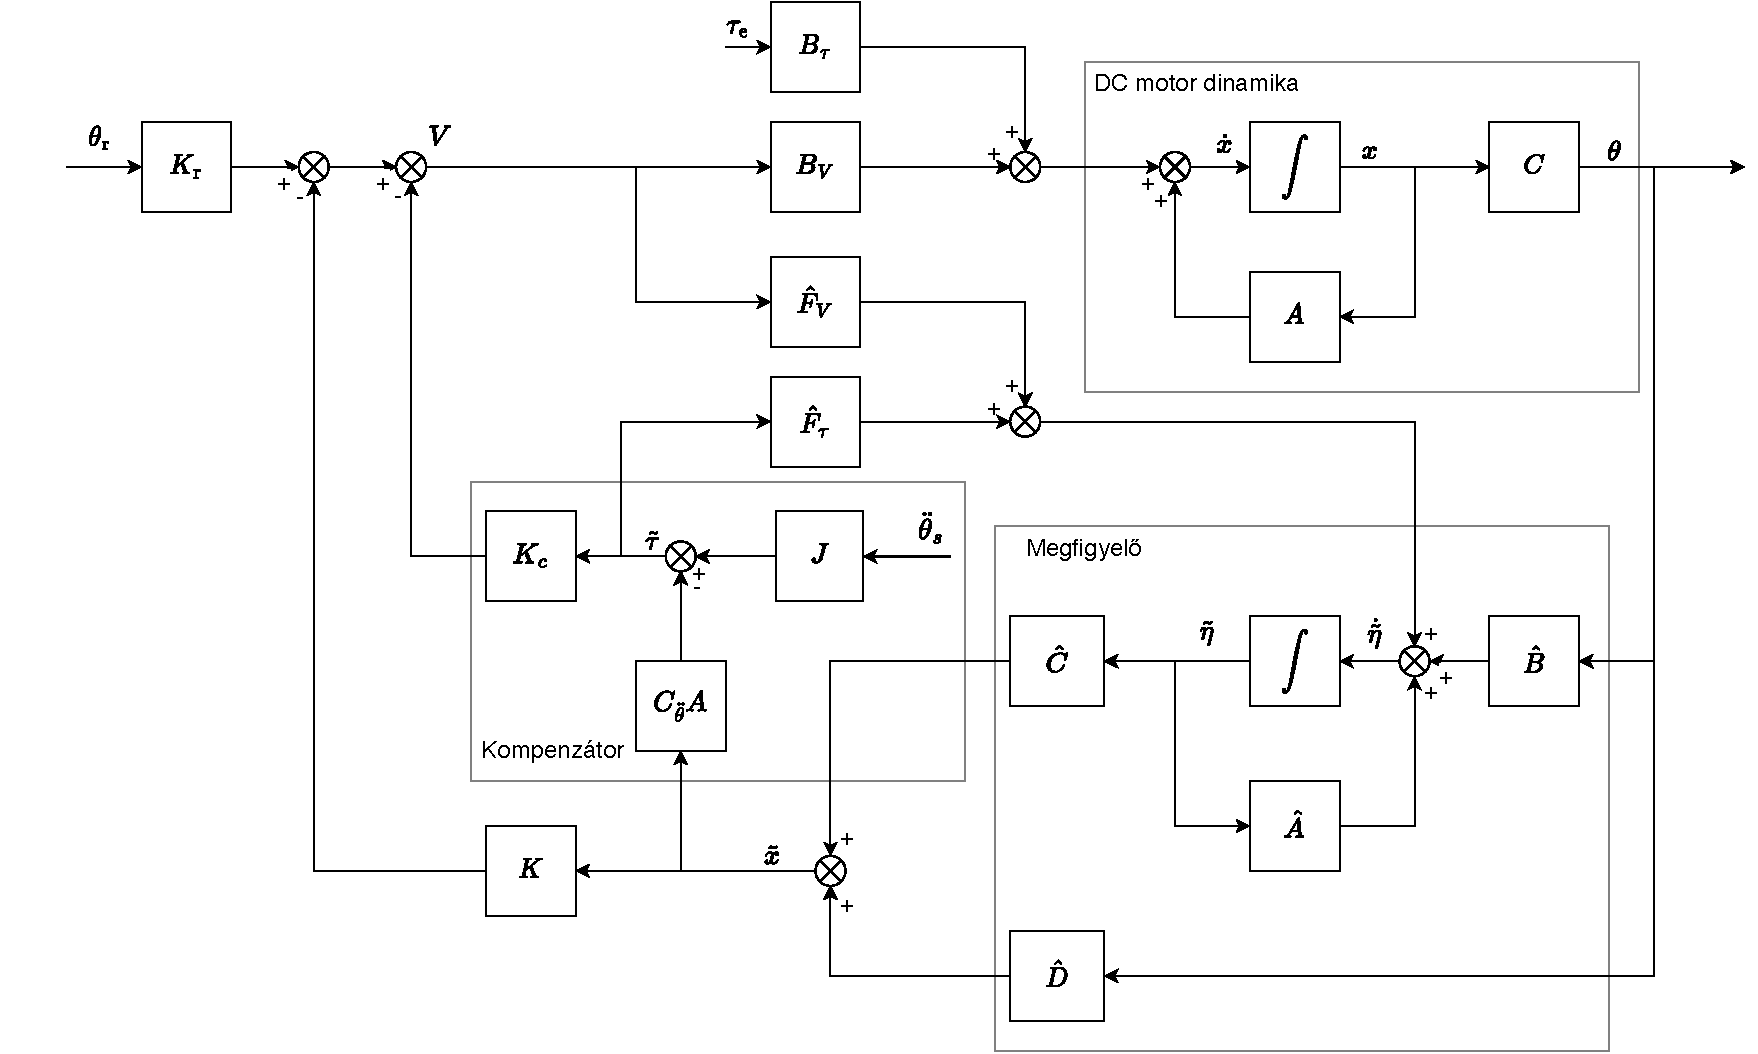
\includegraphics[width=\textwidth]{images/compensated_position_controller_angular_acceleration.pdf}
    \caption{Impedancia szabályozó szöggyorsulás méréssel}\label{fig:block_diagram_indirect_compensation}
    \end{center}
\end{figure}
Ekkor egy becsült nyomaték érték kerül visszacsatolásra, melyeket
\begin{align}
    \tilde \tau = J \ddot \theta_s - \BF C_{\ddot\theta} \BF A \tilde{\BF x}
\end{align}
\begin{align}
    \BF C_{\ddot\theta} = 
    \begin{bmatrix}
        0 & 1 & 0
    \end{bmatrix}
\end{align}
alakban, a becsült állapot és a mért szöggyorsulás kombinációjával adható meg.
A feszültségjel a becsült nyomatékértékkel
\begin{align}
    V = -\BF K \tilde{\BF x} -K_c \tilde \tau + k_1 \theta_r.
\end{align}
Az előző levezetéshez hasonlóan a teljes rendszer dinamikája blokk mátrix alakban
% \begin{align}
%     \begin{bmatrix}
%         \dot{\BF x} \\
%         \dot{\BF e}
%     \end{bmatrix}
%     =
%     \begin{bmatrix}
%         \BF A - \BF B_V \BF K & \BF B_V \BF K \\
%         \BF 0 & \BF A_{bb} - \BF K_e \BF A_{\theta b}
%     \end{bmatrix}
%     \begin{bmatrix}
%         \BF x \\
%         \BF e
%     \end{bmatrix}
%     +
%     \begin{bmatrix}
%         \BF B_\tau - \BF B_V K_c & \BF B_V k_1\\
%         \BF 0 & \BF 0
%     \end{bmatrix}
%     \begin{bmatrix}
%         \tau \\
%         \theta_r
%     \end{bmatrix}.
% \end{align}



Ez a kompenzáció
csak akkor lehet eredményes, ha a rendszer feszültségre és külső nyomatékra 
egyaránt közel azonos sebességgel reagál.
% \begin{figure}[ht]
%     \begin{center}
%     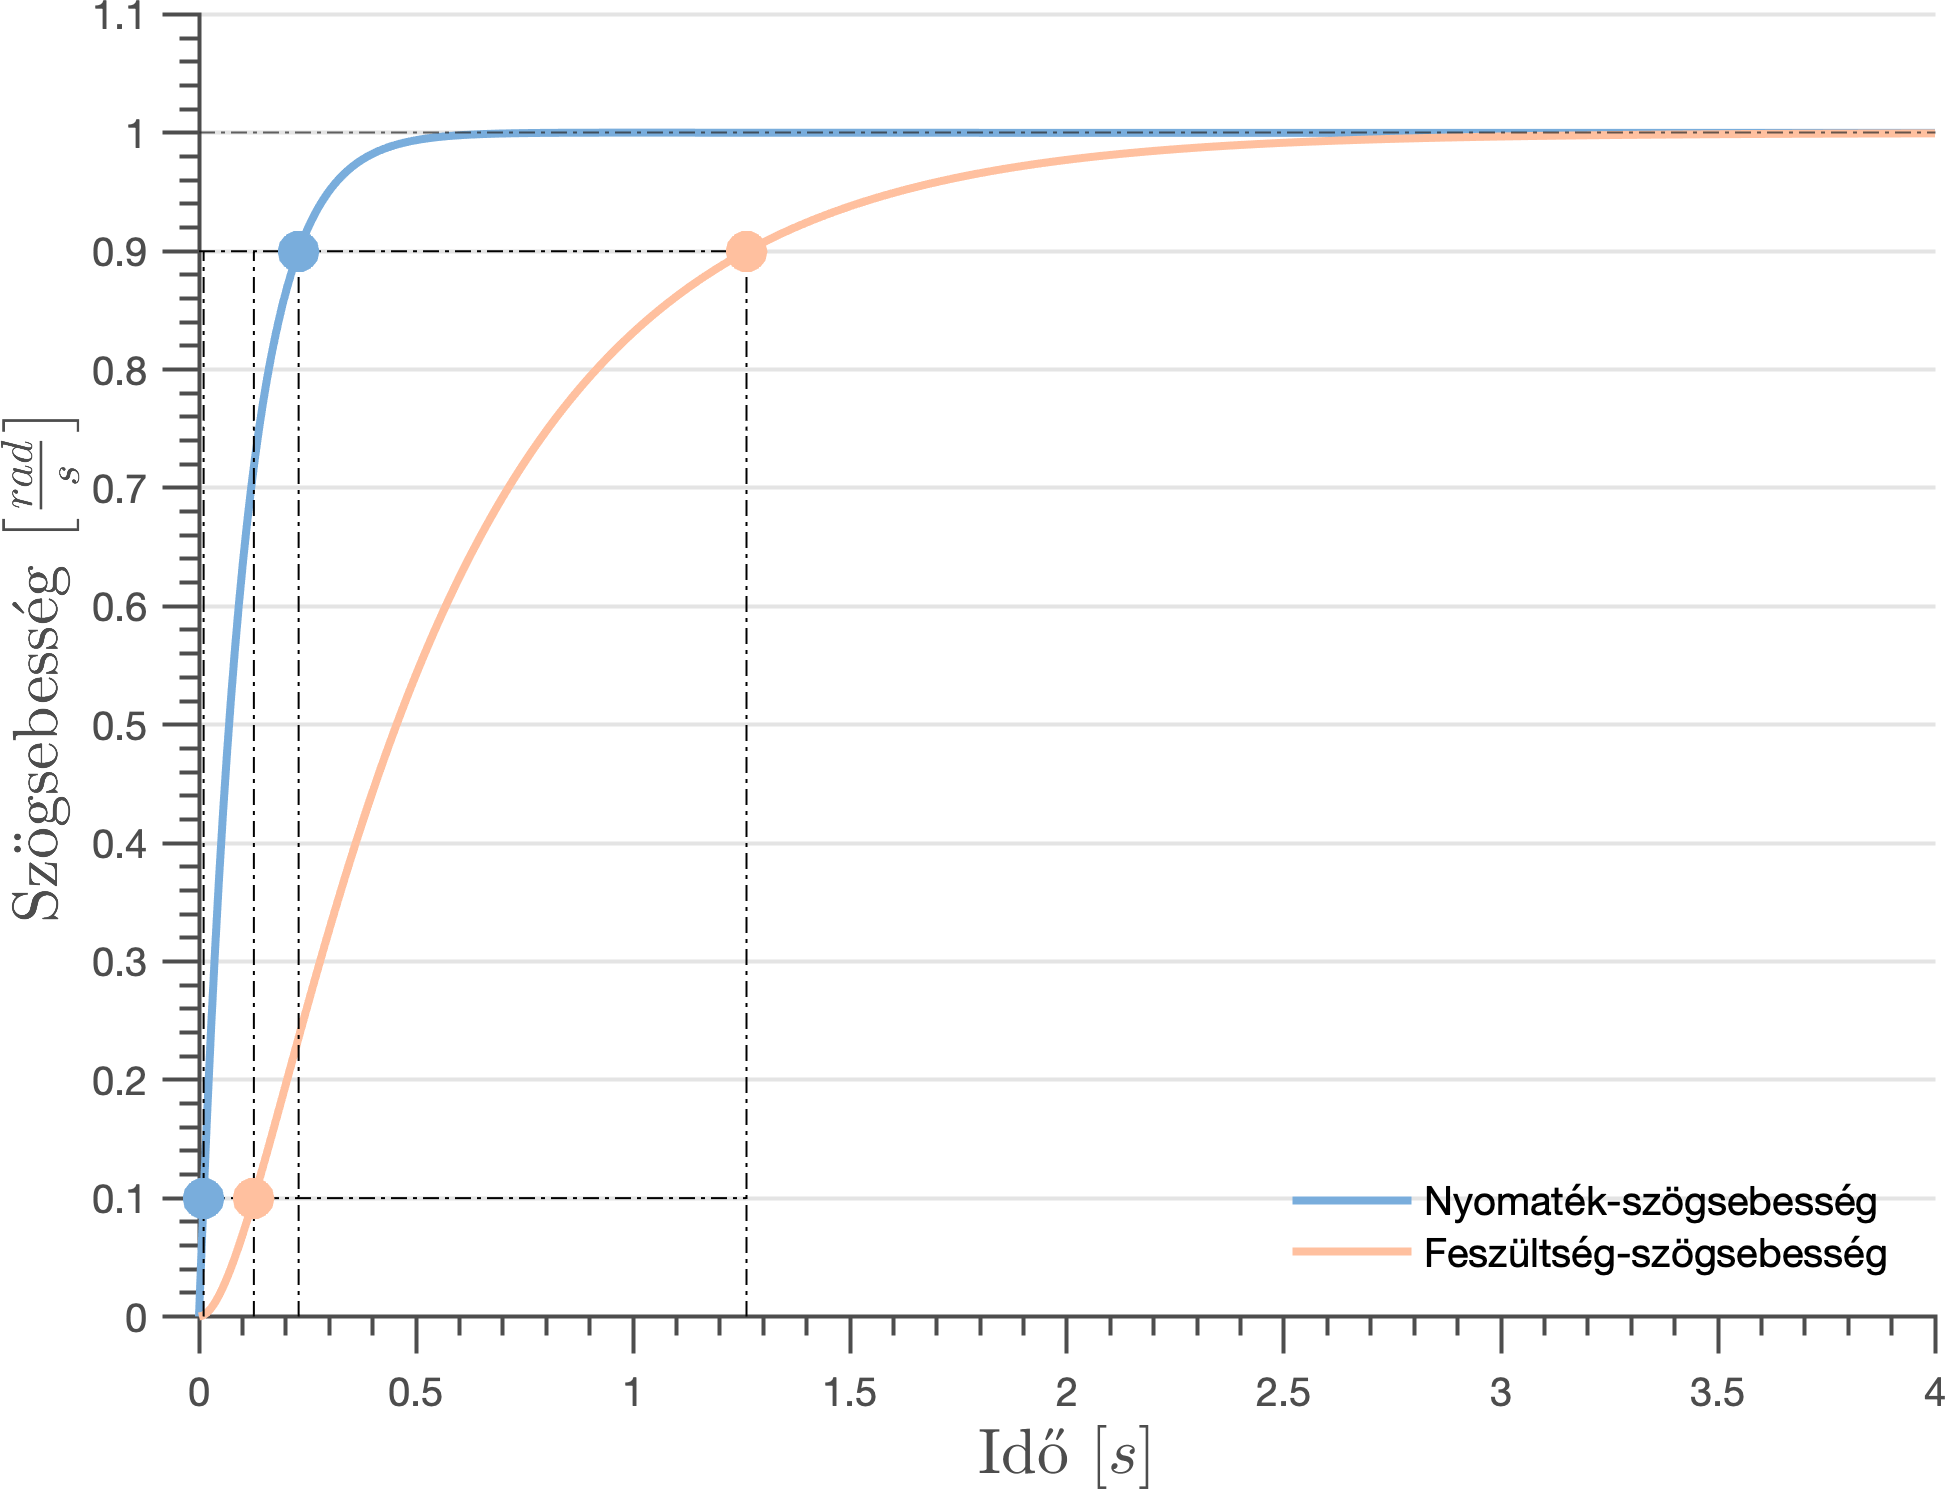
\includegraphics[width=\textwidth]{images/step_response.png}
%     \caption{Külső nyomatékra és feszültségre adott válasz összehasonlítása, 
%     $J = 0.01 \left[kg\cdot m^2\right]$,
%     $K_m = 0.01 \left[kg\cdot \frac{m^2}{s^2}\right]$,
%     $B_m = 0.1 \left[kg\cdot \frac{m^2}{s}\right]$,
%     $L = 0.5 \left[H\right]$,
%     $R = 1 \left[\Omega\right]$}\label{fig:step_response}
%     \end{center}
% \end{figure}
Az eltérő válaszokat szemlélteti~\ref{fig:step_response}-es ábra, mely az~\eqref{eq:transfer_function}-es
egyenletben szereplő átviteli függvények alapján a szögsebesség egységugrásra adott válaszát mutatja. 
A két válasz végértékét egységnyire normalizálva jeleníti meg az ábra a fefutási idő 
összehasonlításának megkönnyítése érdekében. 



\begin{table}%[b!]
    \small\centering
    \caption{Physical parameters of the laboratory rig}
    \label{tab:params}
    \tabcolsep=1pt
    \begin{tabular}{l>{~}l>{\quad}rl}
        \toprule
        \multicolumn{2}{c}{Symbol and parameter name}                                   &                          \multicolumn{2}{c}{Value}                            \\ \midrule
        \(m\)                                                                              & pendulum mass (metal)              &                                0.191 & kg                                     \\
        \(J_{\mathrm{p}}\)                                                                  & pendulum mass moment (metal)         & 5.73\(\cdot\)10\(^{-3}\) & kg\hspace{0.5pt}m\textsuperscript{2}   \\
        \(J_{\mathrm{a}}\)                                                                  & mass moment wrt.~rotor axis (metal)  & 3.027\(\cdot\)10\(^{-3}\) & kg\hspace{0.5pt}m\textsuperscript{2}   \\
        \(m\)                                                                              & pendulum mass  (plastic)               &                                0.134 & kg                                     \\
        \(J_{\mathrm{p}}\)                                                                  & pendulum mass moment (plastic)        & 4.02\(\cdot\)10\(^{-3}\) & kg\hspace{0.5pt}m\textsuperscript{2}   \\
        %        \(J_{\mathrm{a}}\)                                                                  & mass moment wrt.~rotor axis (plastic p.) & 2.92\(\cdot\)10\textsuperscript{-3} & kg\hspace{0.5pt}m\textsuperscript{2}   \\
        \(l\)                                                                              & pendulum half-length         &                                 0.15 & m                                      \\
        \(r\)                                                                              & arm radius                   &                                0.094 & m                                      \\
        \(\tilde{b}_1\)                                                                    & arm combined damping coeff.  &                                1.148 & N\hspace{0.5pt}m\hspace{0.5pt}s        \\
        \(b_2\)                                                                            & pendulum damping coeff.      &                                0.039 & N\hspace{0.5pt}m\hspace{0.5pt}s        \\
        \(C\)                                                                              & pendulum dry friction param. &                                0.011 & N\hspace{0.5pt}m                       \\
        \(N\)                                                                              & motor constant               &                                1.045 & N\hspace{0.5pt}m/V                     \\ 
        \(g\) & gravitational acceleration,          &                                   9.81 & m/s\textsuperscript{2}\\
        
        \(n_{\mathrm{gb}}\) & gearbox ratio & 8523/265 & \\
        %
        \(\lambda_1\) &  \makebox[0pt][l]{{1\textsuperscript{st}}}\phantom{2\textsuperscript{nd}} eigenvalue of system
        matrix \(\mathbf A\) & 4.39                         &                                  s\(^{-1}\) \\ 
        \(\lambda_2\) &        2\textsuperscript{nd} 
        eigenvalue of system
        matrix \(\mathbf A\) & \(-11.09\)                       &                                  s\(^{-1}\) \\
        \(\lambda_3\) & \makebox[0pt][l]{{3\textsuperscript{rd}}}\phantom{2\textsuperscript{nd}}
        eigenvalue of system
        matrix \(\mathbf A\) & \(-656.7\)                       &                                  s\(^{-1}\) \\ 
        \bottomrule
    \end{tabular}
\end{table}


\section{Szabályozó stabilitása}
